% !TeX program = xelatex
\documentclass[UTF8,a4paper,zihao=5,fontset=fandol]{ctexart}
\usepackage[margin=20mm,top=17mm,bottom=18mm]{geometry}
\usepackage{amsmath,amssymb,graphicx,booktabs,array,caption,float,fancyhdr}
\usepackage[hidelinks]{hyperref}
\graphicspath{{figures/}}
\setlength{\parindent}{2em}
\setlength{\parskip}{2pt}
\linespread{1.12}
\ctexset{section={format=\large\bfseries,beforeskip=7pt,afterskip=4pt},
subsection={format=\normalsize\bfseries,beforeskip=5pt,afterskip=3pt}}
\captionsetup{font=small,skip=3pt}
\setlength{\textfloatsep}{6pt}
\setlength{\intextsep}{5pt}
\setlength{\abovedisplayskip}{5pt}
\setlength{\belowdisplayskip}{5pt}
\renewcommand{\arraystretch}{1.15}
\pagestyle{fancy}
\fancyhf{}
\fancyhead[L]{\small 数字图像处理}
\fancyhead[R]{\small Project 1}
\fancyfoot[C]{\small\thepage}
\setlength{\headheight}{14pt}
\renewcommand{\headrulewidth}{0.3pt}
\hypersetup{pdftitle={数字图像处理 Project 1 实验报告},pdfauthor={韩宇、罗云飞、李响}}

\begin{document}
\begin{center}
{\LARGE\bfseries 数字图像处理 Project 1}\par\vspace{5pt}
{\normalsize 第一次 project 实验报告}
\end{center}
\vspace{-4pt}

\noindent\textbf{小组成员与分工}
\begin{center}\small
\begin{tabular}{llp{100mm}}
\toprule
姓名 & 学号 & 代码与报告分工\\
\midrule
韩宇 & 24319050 & Proj03-02: 直方图统计、CDF 映射及均衡化结果分析.\\
罗云飞 & 24307120 & Proj03-05: 二维卷积、拉普拉斯锐化及响应分析.\\
李响 & 24363137 & Proj03-06: 均值滤波、高提升参数比较及结果分析.\\
\bottomrule
\end{tabular}
\end{center}
\vspace{-4pt}

\section{实验目的与环境}
完成直方图均衡化、拉普拉斯锐化和高提升滤波, 比较三种方法的处理结果.
使用 Python 3.13、NumPy、Matplotlib 和 Pillow, 手工实现灰度映射与二维卷积.
空间滤波采用复制边界, 使用 float64 计算; 保存图像时裁剪至 $[0,255]$ 并取整.

\begin{center}\small
\begin{tabular}{llll}
\toprule
实验 & 输入图像 & 尺寸（宽$\times$高） & 通道／灰度范围\\
\midrule
Proj03-02 & 脊柱 MRI & $746\times976$ & RGB／$0\!\sim\!255$\\
Proj03-05 & 月球 & $466\times540$ & RGB／$0\!\sim\!255$\\
Proj03-06 & Fig.3.43(a) & $572\times530$ & 单通道／$0\!\sim\!246$\\
\bottomrule
\end{tabular}
\end{center}
\vspace{-5pt}
前两张图的三个通道数值相同, 统一转为单通道处理.

\section{Proj03-02: 直方图均衡化}
\textbf{方法.} 统计灰度频数 $n_k$, 计算 CDF, 再按映射表逐像素变换:
\[
p_r(k)=\frac{n_k}{MN},\qquad
T(k)=\left\lfloor255\sum_{j=0}^{k}p_r(j)+0.5\right\rfloor,\qquad g=T(f).
\]
采用四舍五入, 不减去最小非零 CDF. 整数累计频数用于保证半整数处的取整准确.

\begin{figure}[H]
\centering
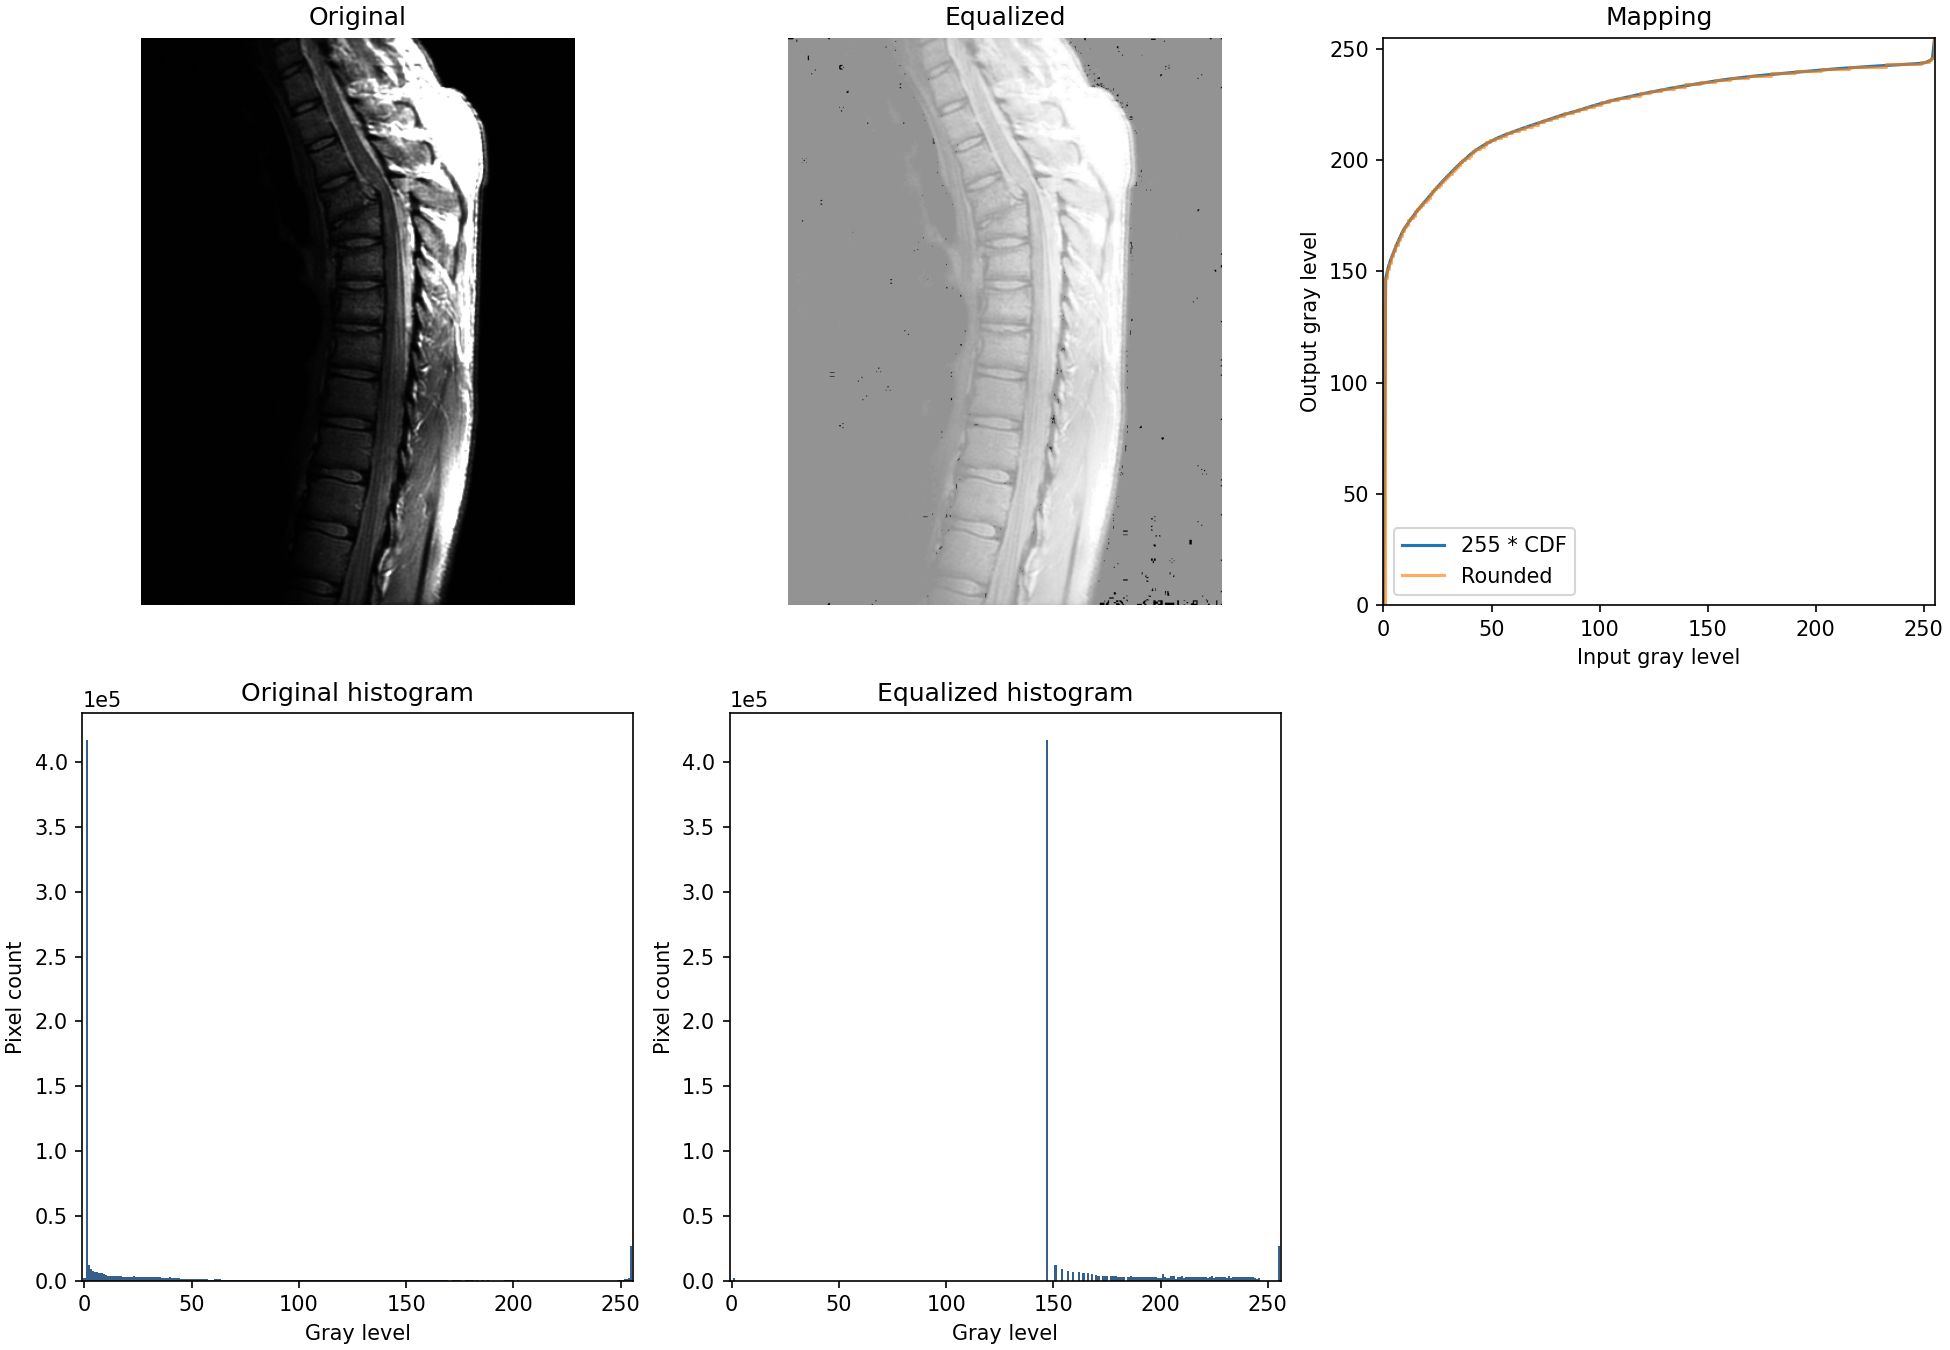
\includegraphics[width=0.79\linewidth]{p32_summary.png}
\caption{直方图均衡化结果: 原图、输出图、映射曲线及前后直方图.}
\end{figure}

\textbf{结果.} 原图中灰度不超过 30 的像素占 75.76\%, 暗部层次不明显.
均衡化后椎体轮廓更容易辨认, 平均灰度由 32.64 变为 169.90.
占比 57.23\% 的灰度 1 被映射到 147, 因此背景大面积变灰.
相同输入灰度不能拆分, 加上取整合并, 输出仍有明显尖峰, 实际灰度级由 256 降为 85.

\newpage
\section{Proj03-05: 拉普拉斯锐化}
\textbf{方法.} 使用正中心八邻域模板, 先计算带符号响应, 再与原图相加:
\[
K=\begin{bmatrix}-1&-1&-1\\-1&8&-1\\-1&-1&-1\end{bmatrix},\qquad
R=K*f,\qquad g=f+R.
\]
卷积结果保留负值. 响应灰度显示图采用线性缩放, 显示用缩放不参与锐化计算.

\begin{figure}[H]
\centering
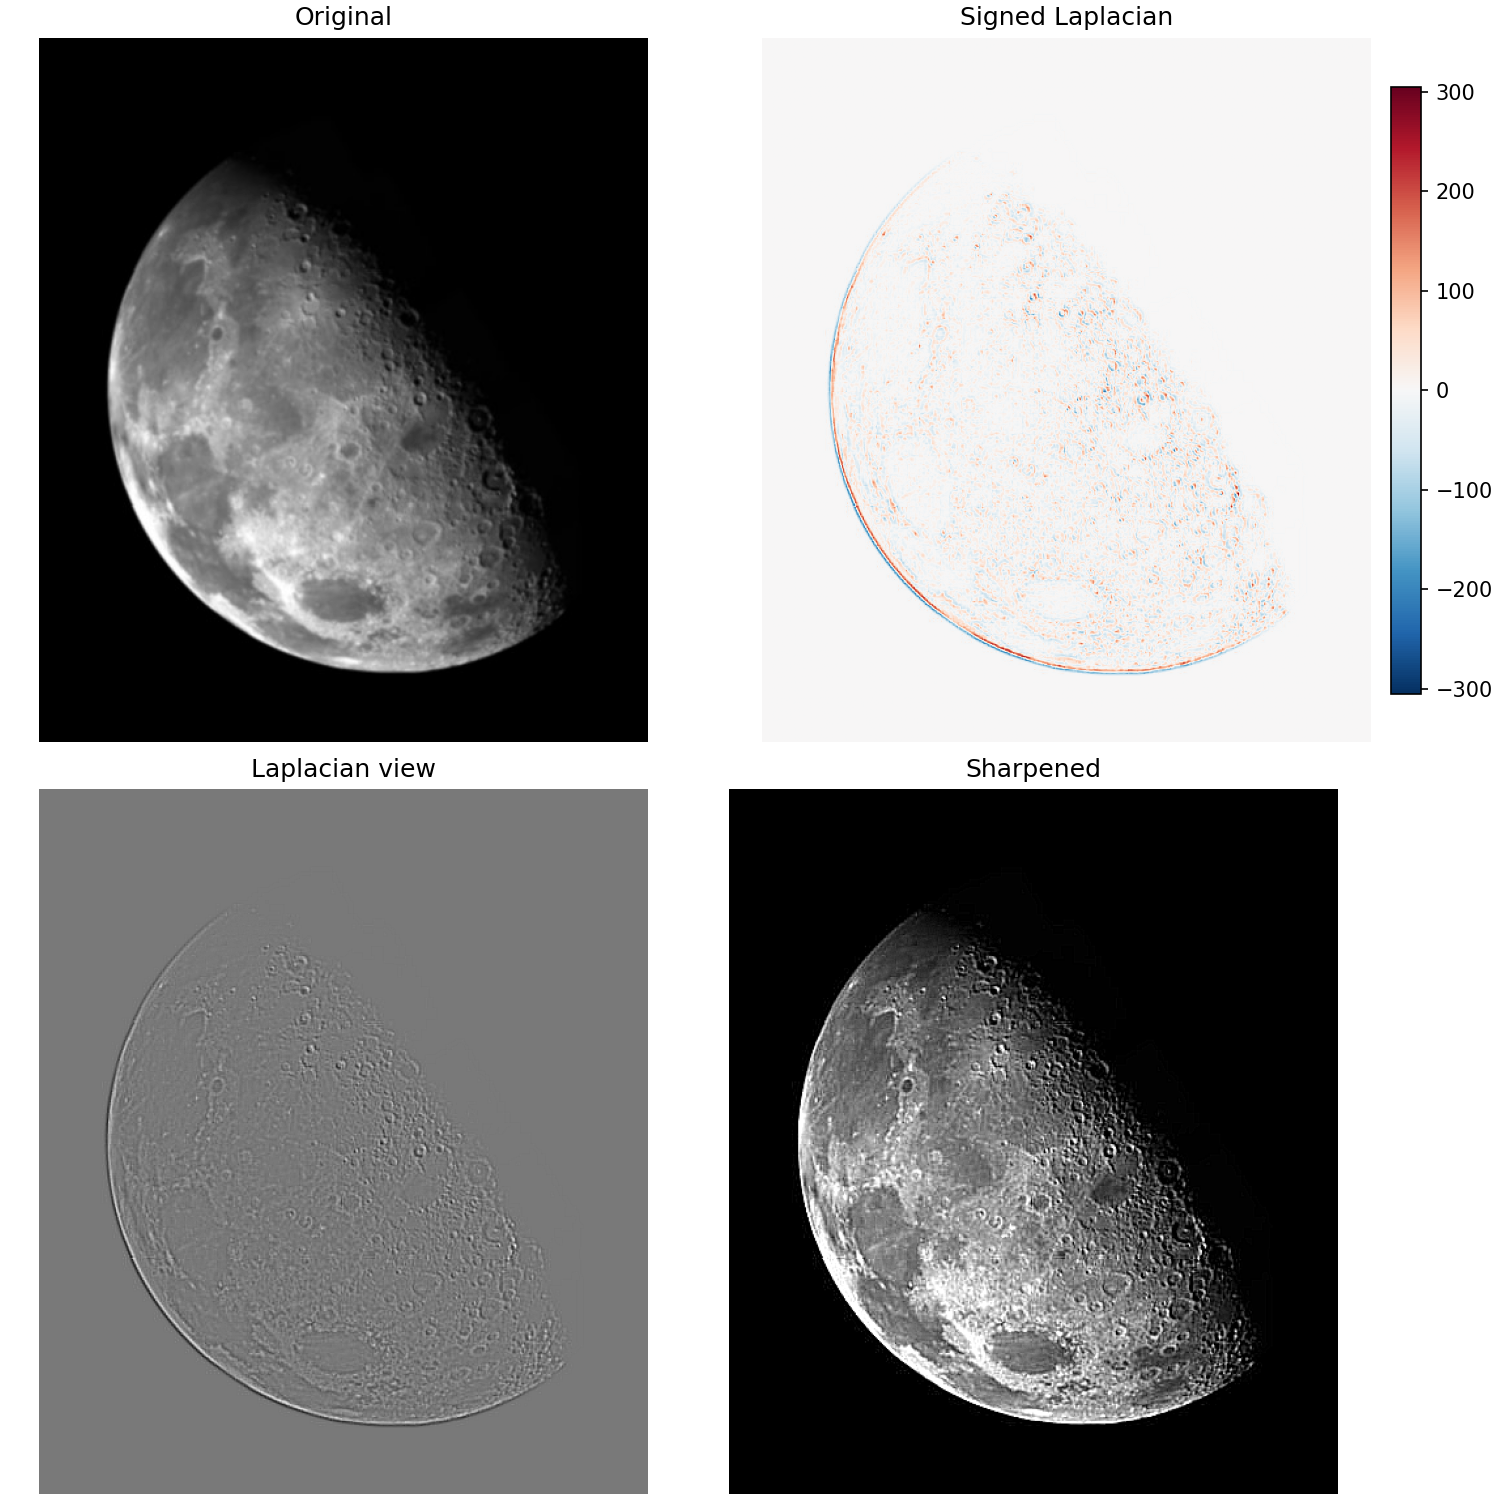
\includegraphics[width=0.70\linewidth]{p35_summary.png}
\caption{月球锐化: 原图、带符号响应、线性缩放响应和锐化图.}
\end{figure}

\begin{figure}[H]
\centering
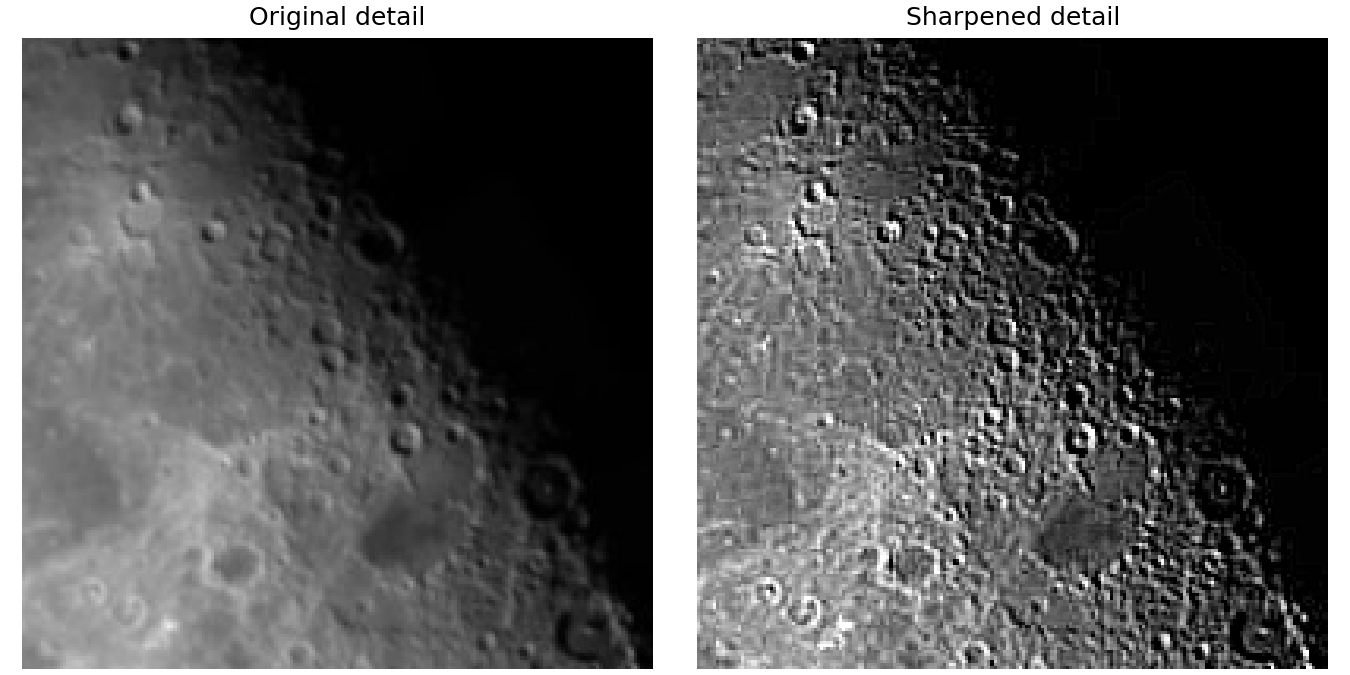
\includegraphics[width=0.60\linewidth]{p35_detail.png}
\caption{同一局部的锐化前后比较, 左为原图, 右为锐化结果.}
\end{figure}

\textbf{结果.} 平坦区响应接近 0, 月球边缘和环形山轮廓响应较大.
相加后边缘的明暗差增大, 轮廓变清楚, 但颗粒感和亮线也更明显.
响应范围为 $[-274,305]$, 相加后为 $[-251,485]$;
裁剪前低于 0 和高于 255 的像素分别占 3.93\% 和 1.00\%.
结果符合教材的锐化趋势; 由于未提供 Fig.3.40 的完整结果图, 未作逐像素比较.

\newpage
\section{Proj03-06: 非锐化掩模与高提升滤波}
\textbf{方法.} 用 $3\times3$ 均值模板计算模糊图, 再按题目公式处理:
\[
B=\frac19\begin{bmatrix}1&1&1\\1&1&1\\1&1&1\end{bmatrix},\quad
\bar f=B*f,\quad m=f-\bar f,\quad H_A=Af-\bar f=(A-1)f+m.
\]
\begin{figure}[H]
\centering
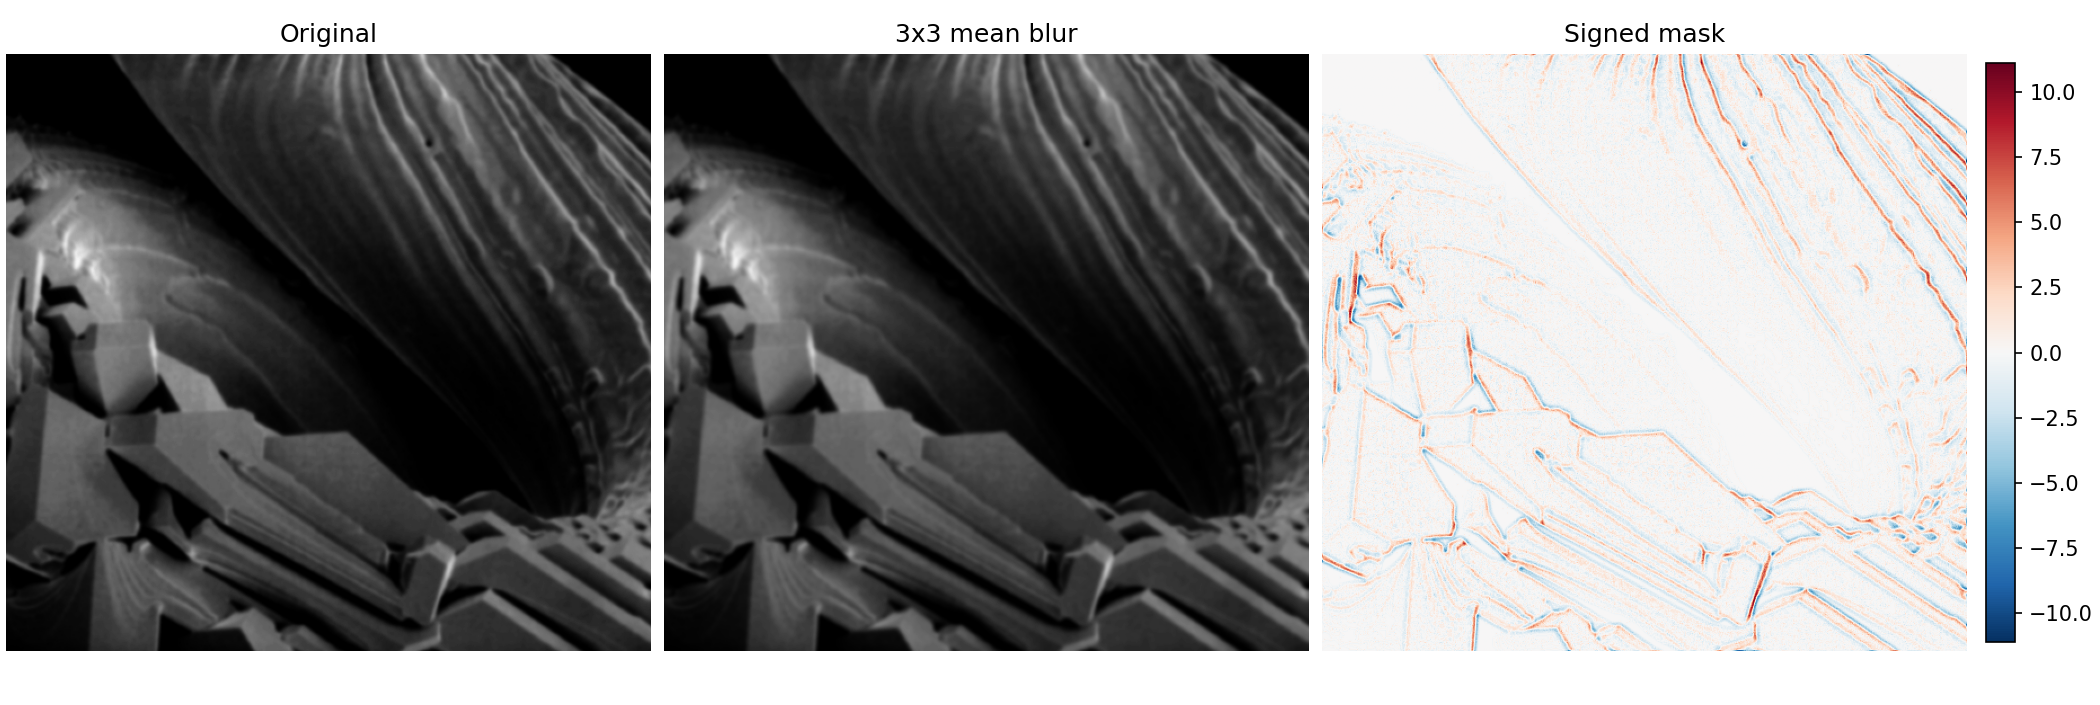
\includegraphics[width=\linewidth]{p36_steps.png}
\caption{原图、均值模糊图和带符号掩模. 掩模范围为 $[-10.78,11.11]$.}
\end{figure}

\textbf{参数比较.} 先测试六个指定值, 所有候选统一按 $[0,255]$ 裁剪显示.
\begin{figure}[H]
\centering
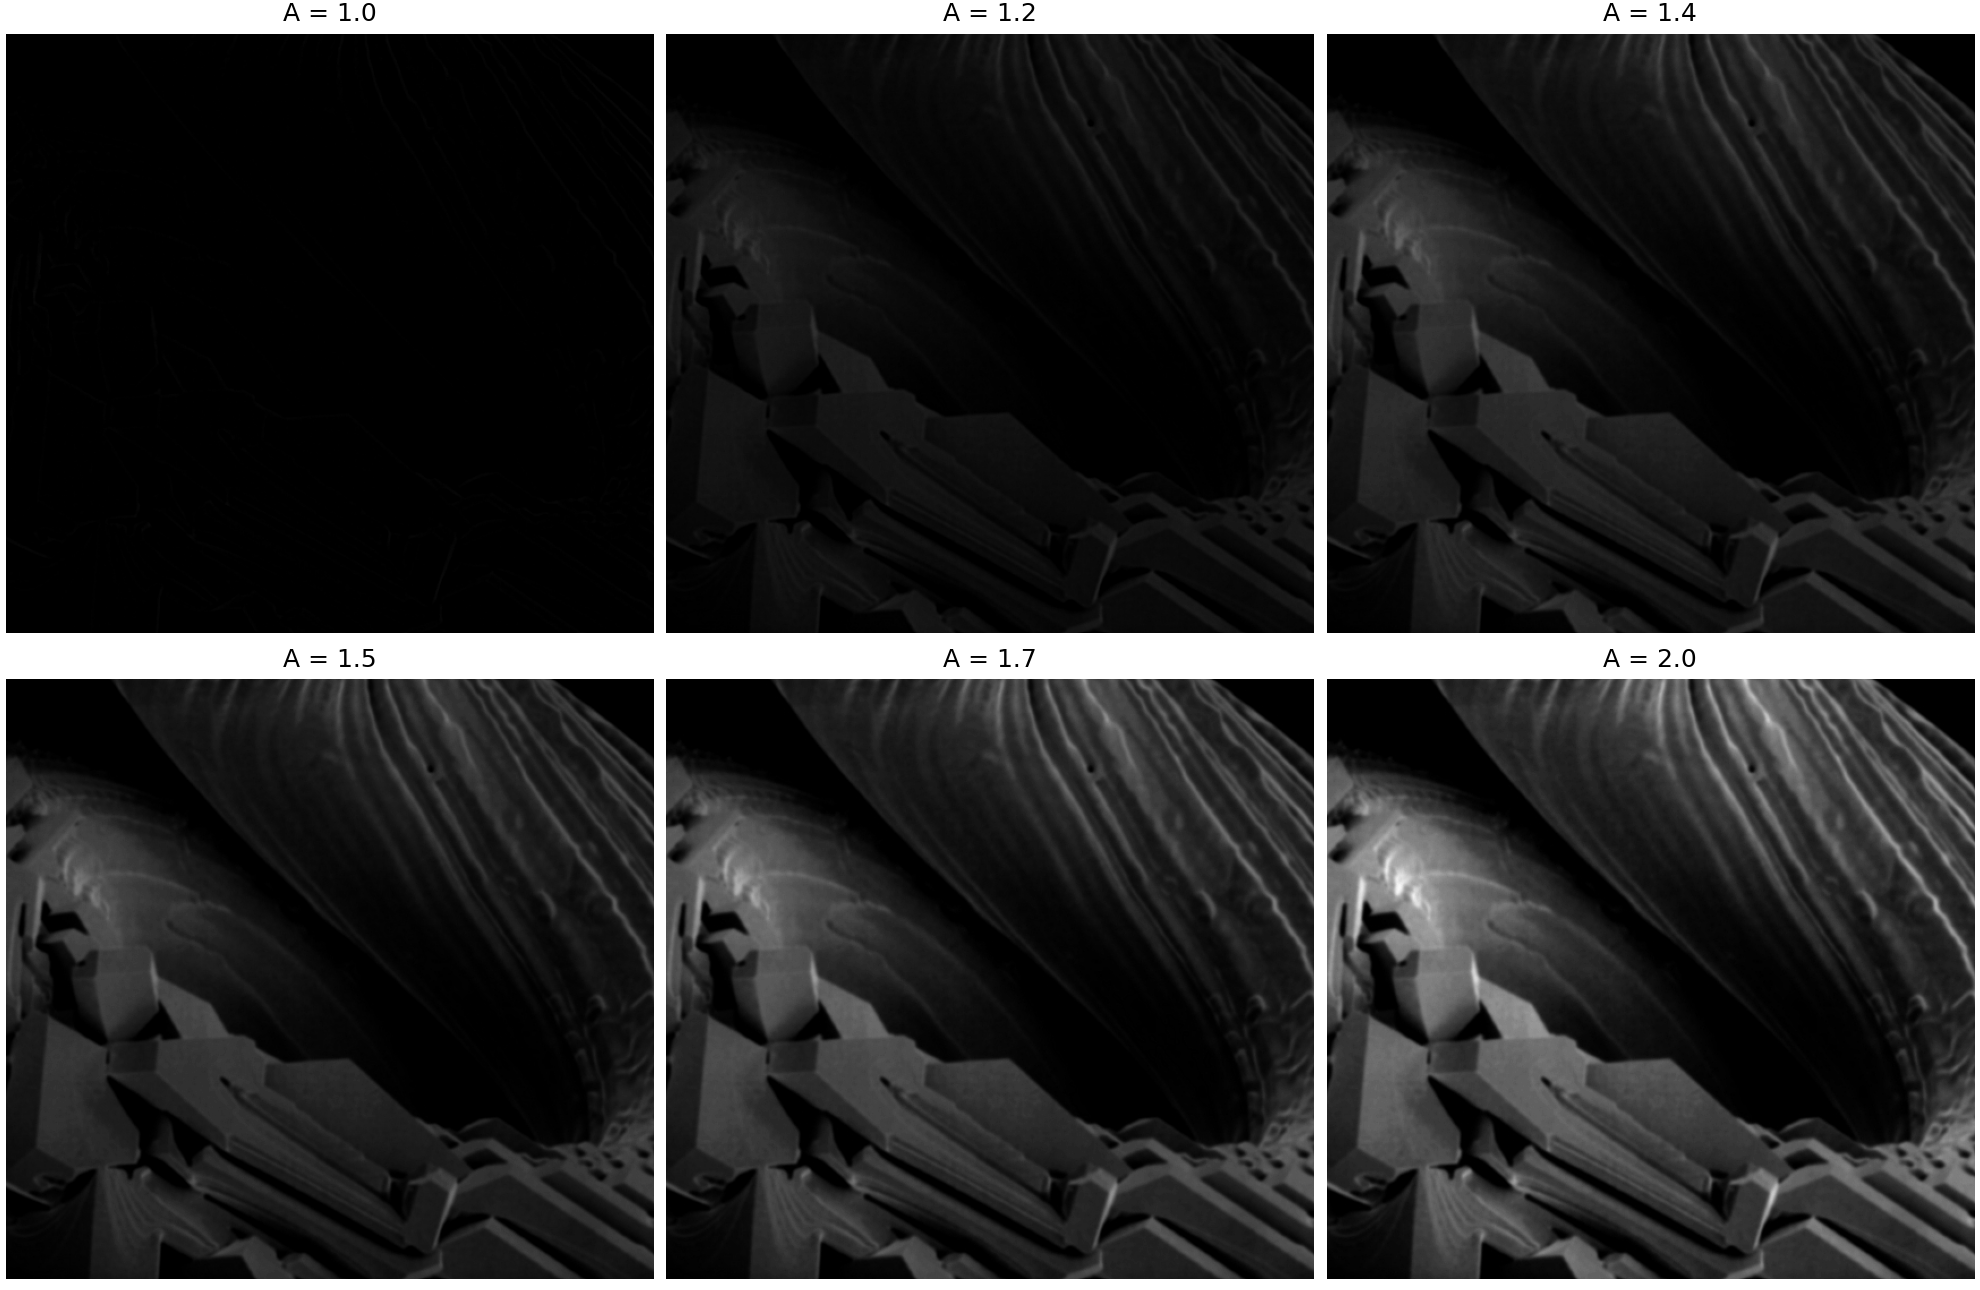
\includegraphics[width=\linewidth]{p36_compare_main.png}
\caption{指定参数 $A=1.0,1.2,1.4,1.5,1.7,2.0$ 的结果.}
\end{figure}

$A=1$ 时只有掩模, 直接显示几乎全黑; $1<A<2$ 时整体偏暗;
$A=2$ 时为通常的非锐化锐化 $f+m$, 亮度接近原图.
由于参考图更亮, 继续补测 $A=2.2,2.5,2.7,3.0$.

题目公式中增大 $A$ 改变的是原图项, 掩模系数仍为 1.
教材 Fig.3.43 的同名参数采用另一种定义, 不能直接将其 $A=1.7$ 用于本式.
在本次模板下, $K*f=9m$, 两种方法的细节增强量也不同.

\newpage
\subsection*{补充比较与最终选择}
\begin{figure}[H]
\centering
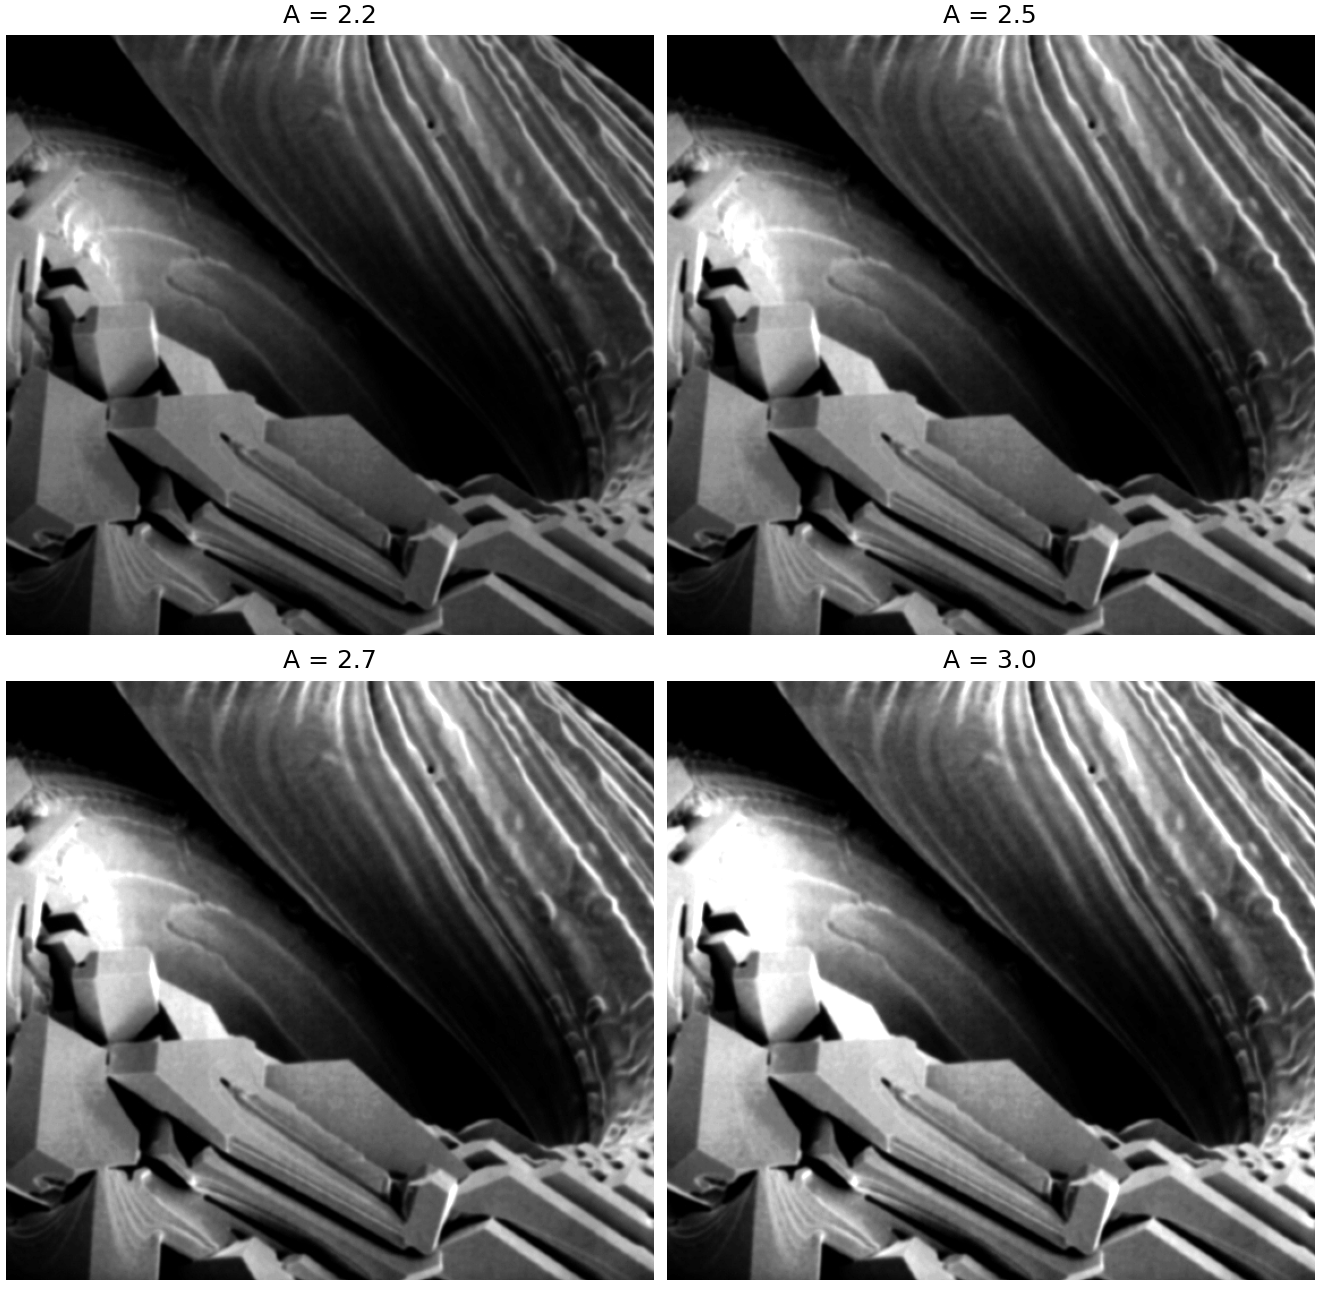
\includegraphics[width=0.63\linewidth]{p36_compare_extra.png}
\caption{补充参数比较, 左下为最终选定的 $A=2.7$.}
\end{figure}

\noindent\begin{minipage}[t]{0.47\linewidth}
\centering\small
\vspace{0pt}
\begin{tabular}{rrr}
\toprule
$A$ & 输出均值 & 高端越界比例\\
\midrule
1.0 & 0.36 & 0.00\%\\
1.2 & 10.10 & 0.00\%\\
1.4 & 20.15 & 0.00\%\\
1.5 & 25.21 & 0.00\%\\
1.7 & 35.26 & 0.00\%\\
2.0 & 50.35 & 0.00\%\\
2.2 & 60.41 & 0.10\%\\
2.5 & 75.38 & 0.47\%\\
\textbf{2.7} & \textbf{85.15} & \textbf{1.26\%}\\
3.0 & 99.07 & 3.94\%\\
\bottomrule
\end{tabular}
\par\vspace{3pt}\footnotesize
均值按保存图像统计; 高端越界指裁剪前大于 255 的像素.
\end{minipage}\hfill
\begin{minipage}[t]{0.49\linewidth}
\vspace{0pt}\centering
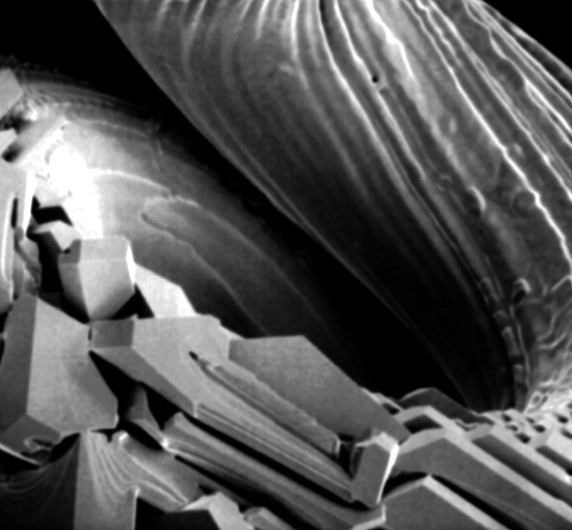
\includegraphics[width=0.89\linewidth]{p36_final.png}
\captionof{figure}{$A=2.7$ 的最终结果.}
\end{minipage}

\textbf{选择.} $A=2.7$ 的条纹和构件亮度较接近参考图.
$A=3.0$ 的亮区发白更多, 高端越界比例增至 3.94\%, 因此选用 $A=2.7$.
该参数按视觉效果确定, 仍有局部饱和, 不能精确复现教材结果.
过大的增益容易造成过冲、噪声增强和亮部层次丢失.

\section{实现中的处理与总结}
用整数累计频数避免 CDF 半整数取整误差; 卷积按核元素累加数组切片,
不逐像素执行 Python 循环. 保留带负值响应, 并用相同显示范围比较参数, 避免显示拉伸干扰判断.
均衡化展开了暗部层次, 同时抬高背景; 拉普拉斯使轮廓更清楚, 但带来过冲;
高提升最终选用 $A=2.7$. 程序保存全部中间结果, 原有 75 项数值检查均通过.
本次没有进行速度或泛化性基准测试.

\vspace{2pt}\noindent{\footnotesize
参考: Gonzalez \& Woods, \textit{Digital Image Processing}, Fourth Edition; 课程提供的实验要求及参考图.}
\end{document}
